\chapter{KG-RNN: Our Architecture}
\label{chap:KG-RNN}
In this chapter we introduce our own architecture, based on the previous chapter where we present our \textbf{Evolving Entity Encoder}. This novel architecture leverage different graph theory techniques and machine learning to encompass information from other entities and thus further boost the predictive power of the model. \\

The first section will highlight the different steps of the pipeline, then the following section describes the process of constructing the weighted knowledge graph from internal (MIMIC-III) as well as external information. Right after, we develop the idea of ``extracting`` other entities of interest from the knowledge graph that will improve the prediction for a given input entity. Finally, we expose our \emph{KG-RNN} deep learning architecture to leverage the input entity as well as the ones we extracted in the previous stage.

\section{Overview}
Our ``KG-RNN`` architecture extends on the previous baseline described in chapter~\ref{chap:Baseline}. The novelty and improvement rely on neighboring entities of interest (i.e. admissions in our use-case) to encompass more information than solely the input entity. \\

To do so, the first phase consists in creating an appropriate knowledge graph from our dataset but also external information to enrich the linkage structure between entities. This can be done in many different ways, in a weighted or unweighted fashion ($w=1$), and we will describe here how we proceeded in the healthcare use-case. \\

Right after, from this enhanced knowledge graph, weighted or not, we have to extract neighboring entities of interest. For this purpose, we can employ any graph sampling technique (leveraging edge weight or not) and we will go through the one we chose. Finally, from the extracted neighbors and the input entity, we build a machine learning model extending from the baseline one to convey information from these neighbors.

\section{Weighted Knowledge Graph Construction}
As a first step and to the end of building our weighted knowledge graph, the main field of interest is~\emph{DIAGNOSIS} (that we will call ``prediagnosis`` hereafter to avoid confusion with ICD9 diagnoses) in the admission table. Firstly, we clean the prediagnosis: \begin{enumerate*}\item Converting to lower-case. \item Remove non-alphabetic characters. \item Remove multi-spaced as well as leading and trailing ones.\end{enumerate*} \\

On top of this \textit{prediagnosis}, we leverage external information from a recent paper that creates a mapping between diseases and symptoms~\cite{Rotmensch2017}. This external knowledge graph is built from Electronic Health Records (EHR) and links diseases with their respective symptoms, while providing a symptom relevance weight (between 0 and 1). An example of entry from this external source is: \emph{Migraine: Headache ($w=0.384$), nausea ($w=0.316$), sensitivity to light ($w=0.223$), ...} These diseases and symptoms are cleaned in the exact same way as the prediagnosis and assembled to create our \textbf{dictionary}. \\ 

Our goal now is to link the external information with our internal information to create an enriched knowledge graph. We want to link prediagnosis with symptoms and diseases, while these latter two are intrinsically linked directly by the external information (cf. \textit{Migrain} example above). \\

To this end we have to cope with the problem of spelling mistakes as well as quasi-similar prediagnosis and diseases/symptoms (e.g. ``Coronary heart disease`` vs. ``Arteries heart disease``), we create a character N-grams~\footnote{\url{https://en.wikipedia.org/wiki/N-gram}} (where the size of the n-gram has to be tuned) list from the cleaned entries of the dictionary (prediagnosis, disease and symptoms). From this n-grams list, we create a TF-IDF~\footnote{\href{https://en.wikipedia.org/wiki/Tf\%E2\%80\%93idf}{https://en.wikipedia.org/wiki/Tf\_idf}} vector with a minimum document frequency of 1. \\

Finally, we match prediagnosis with diseases and symptoms based on the cosine similarity between their n-grams + TF-IDF vectors. Namely, we link a prediagnosis with a disease and a symptom if their cosine similarity score is above a given threshold (to manually filter out noise), and we link diseases and symptoms based on the external information while also applying a threshold on the symptoms relevance weight provided out-of-the-box by the external source. The final knowledge graph is represented in the figure~\ref{fig:kg-healthcare}, including both internal and external information. \\

\begin{figure}[H]
 \centering
 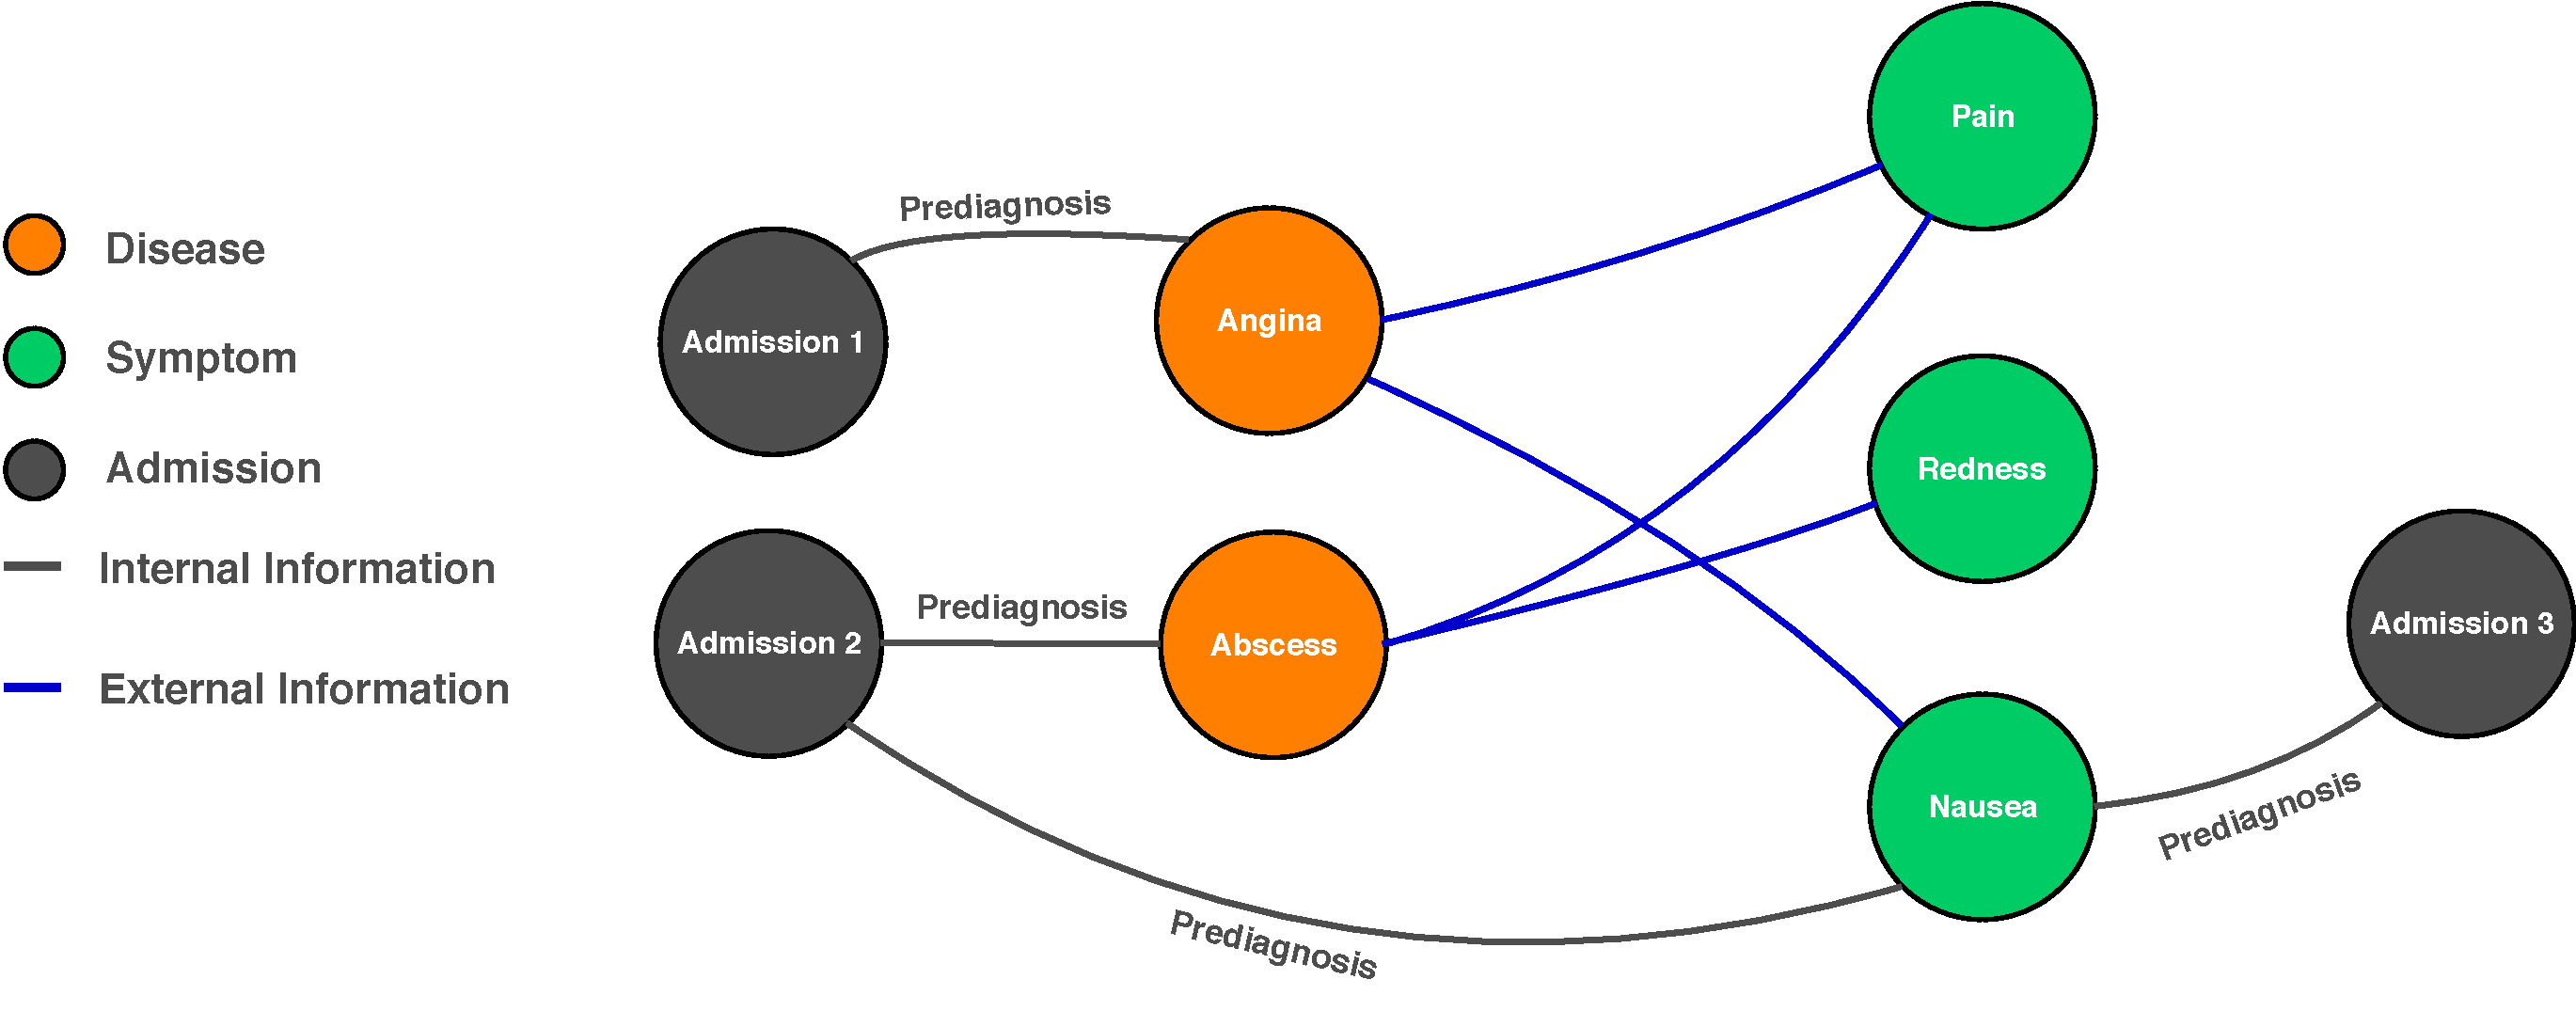
\includegraphics[width=0.9\textwidth]{figures/kg-healthcare.pdf}
 \caption{Final knowledge graph made of external and internal information that will be used in the experiments and discussions.}
 \label{fig:kg-healthcare}
\end{figure}

On a practical note, for the rest of the discussions and experiments, we set n-grams to \textbf{3 characters}, the minimum cosine similarity score of \textbf{0.6} and a relevance weight between diseases and symptoms of \textbf{0.2}.

\newpage
\section{Weighted Knowledge Graph Extraction}
Secondly, from this weighted knowledge graph, we want to extract relevant neighboring entities to enrich our input entity with additional information. For this purpose, one can use any graph sampling technique~\cite{DBLP:journals/corr/HuL13, Leskovec:2006:SLG:1150402.1150479}, making use of the weights defined during \textit{Graph Construction} or not. \\

This graph sampling will be very important for the downstream model and also the number of neighbors is a critical hyper-parameter that has to be tuned. In that regard, relevant experiments can be found in the appropriate chapter. Some common sampling techniques could be \begin{enumerate*}\item Random sampling on 1-hop neighbors. \item Snow-Ball sampling. \item Forest Fire sampling.\end{enumerate*}. \\

For our use-case at hand, we decided to employ some \textit{importance sampling} based algorithm. This technique is inspired from a paper~\cite{DBLP:journals/corr/abs-1806-01973} by Pinterest and Stanford, it relies on random walks to create an importance score for each entity and take the top scoring entities as neighbors of interest. \\

Concretely, the process is to simulate many random walks \emph{starting from input entity} and compute the $L_1$-normalized visit count as the importance score. Now, instead of simulating thousands of random walks it can be proven that in the limit of an infinity of simulations, the normalized $L_1$ visit count is equivalent to a Personalized PageRank score. Henceforth, we decided to compute the Weighted Personalized PageRank score (personalized on the input entity) using \textit{Oracle PGX} for each input entity. \\

Finally, and as stated previously, the top-$M$ scoring entities are extracted for each input admission and we define a minimum score of \textbf{0.0001} as an arbitrary threshold. Otherwise, there would always have exactly M neighbors sampled even if some are isolated and thus have a score of 0. This threshold allows for more flexibility and to have $0 \leq \mbox{neighbors} \leq M$ for a given input admission. A made-up example resulting from this whole process is available in figure~\ref{fig:kg-healthcare-extraction}.\\

From a practical standpoint, we also make sure not to sample neighbors from the testing or validation set when we are training, or respectively sampling entities from the training or testing set during validation. Equivalently, we make sure not to sample entities from training and validation when we do the final evaluation on the test set.

\begin{figure}[H]
	\centering
	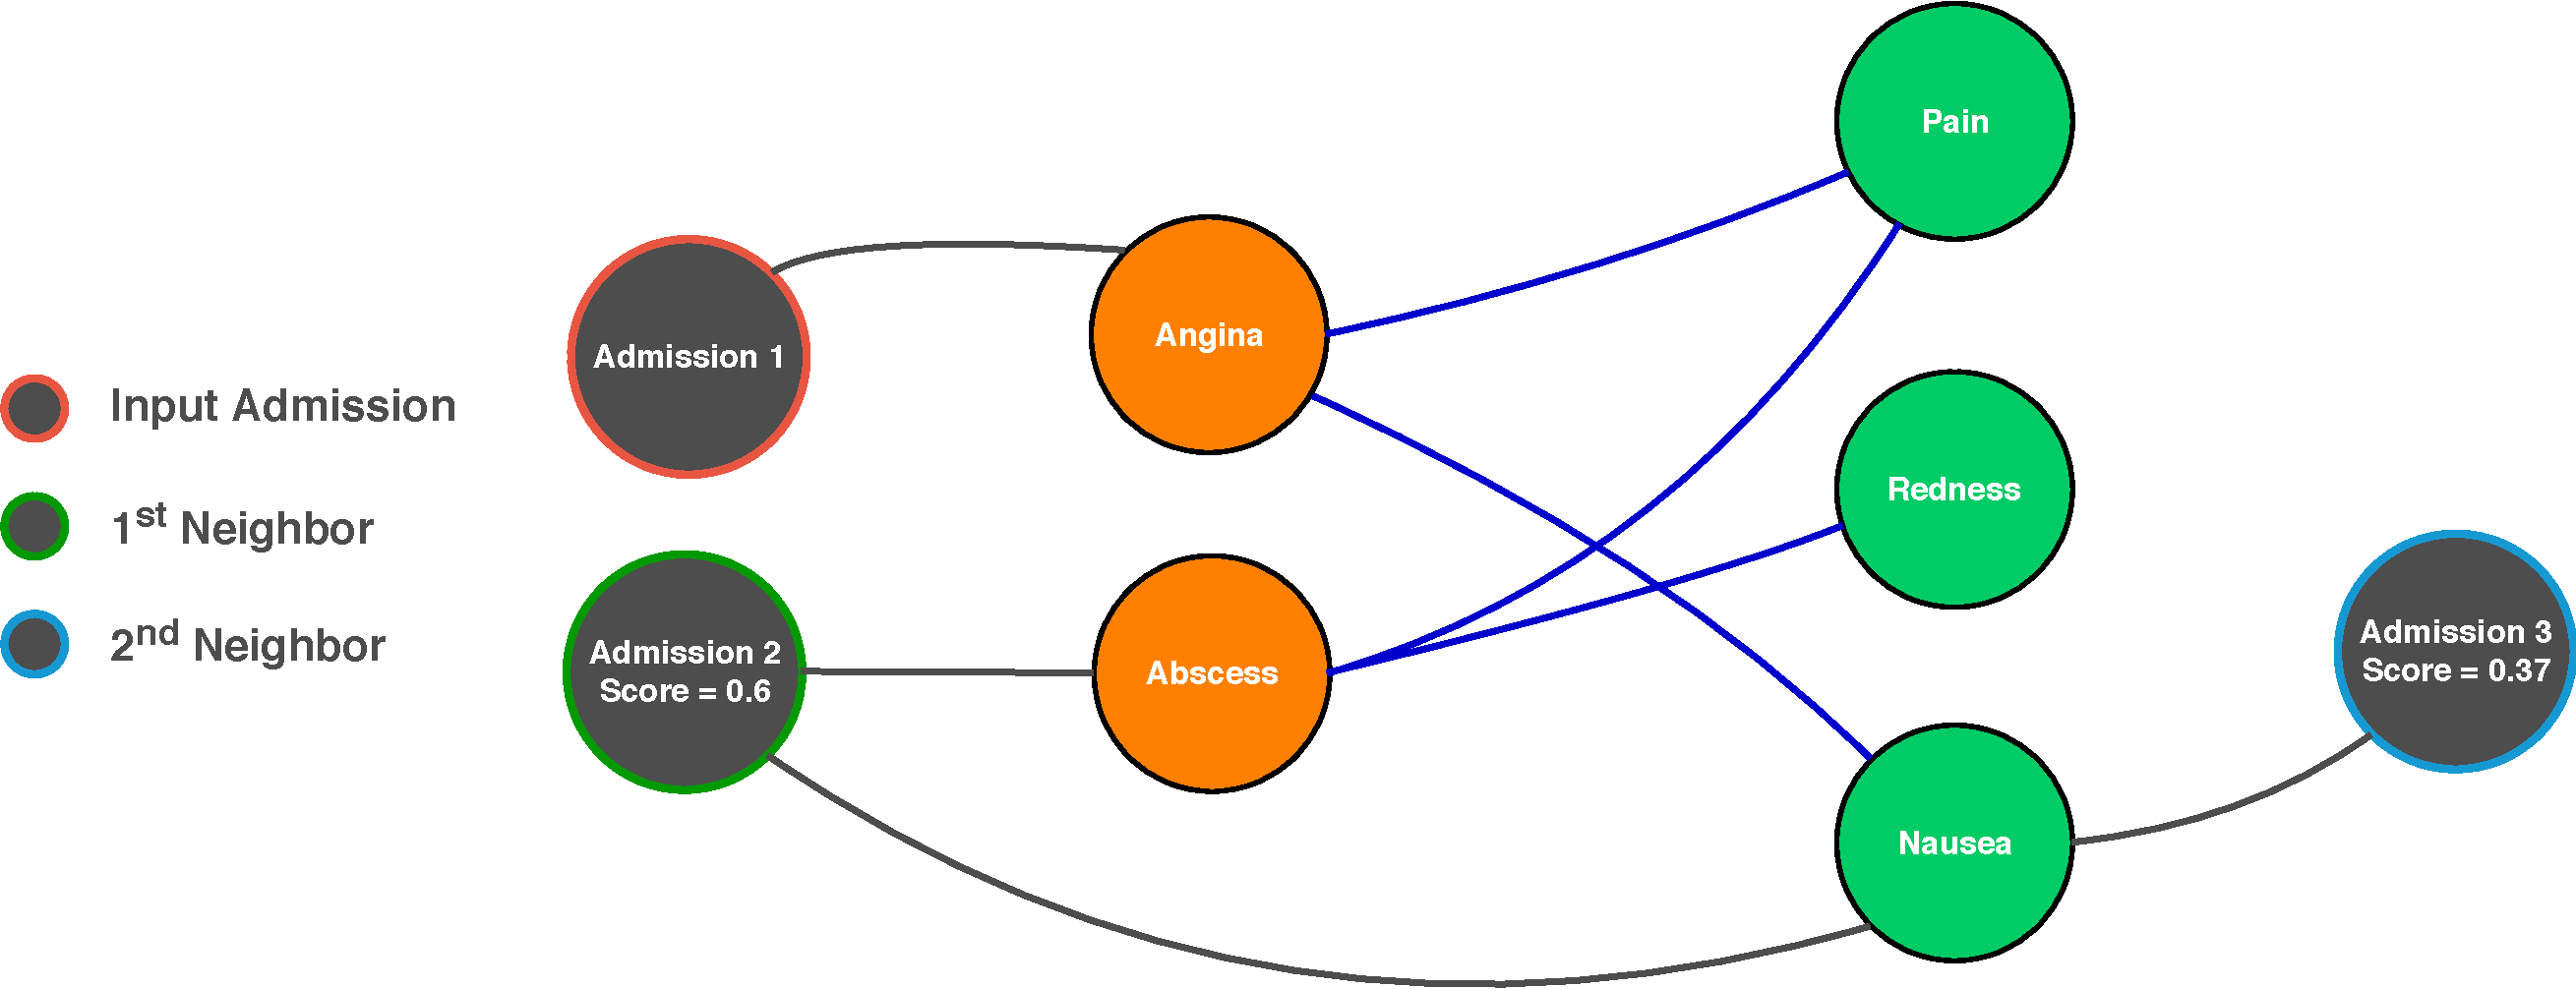
\includegraphics[width=0.9\textwidth]{figures/kg-healthcare-extraction.pdf}
	\caption{Example of potential \textit{WPPR} scoring for the knowledge graph in figure~\ref{fig:kg-healthcare}. If we set $M=1$, only ``Admission 2`` would be extracted, whereas if we set $M=2$ both admissions 1 and 2 would be extracted as neighbors of ``Admission 1``.}
	\label{fig:kg-healthcare-extraction}
\end{figure}

\newpage
\section{Graph Machine Learning}
The machine learning model encapsulating information from neighboring entities as well as the input entity relies on the building block described in the chapter~\ref{chap:Baseline}. Indeed, the input admission is first encoded using the \textbf{Evolving Entity Encoder} from which the final embedding vector $\bm{\tilde{h}} \in \mathbb{R}^{b}$ is fed to the main module. The main module job lies in blending information from extracted neighbors with the input admission vector $\bm{\tilde{h}}_i^m$. \\

To better understand the mechanics, the extracted neighbors can be seen as made of static information throughout admission (e.g. patient age) and dynamic information (e.g. their respective events). The main module can either process dynamic information and static information, or just one or the other. Explicitly, the extracted neighbors entities can also go through the Evolving Entity Encoder to embed their dynamic behavior in a vector $\bm{\tilde{h}} \in \mathbb{R}^{b}$ that will be then concatenated with static information vectors. \\

Eventually, the embedded vector is concatenated with static information vectors, and fed through a fully-connected layer (\textit{encoder}) to obtain the final neighbor encoding vector. These vectors are then fed through an aggregator of the same kind as the one described in chapter~\ref{chap:Baseline}, that is \textit{sum}, \textit{mean} or \textit{max}. hHe purpose of this aggregator is to squash the data along the $M$ dimension to squeeze out information from neighbors. The final prediction diagnoses are made from the concatenation of the aggregated neighbors and input entity encoding, that is finally fed into a fully-connected layer mapping to our \emph{50} classes. \\

On our use-case at hand, we decided to discard dynamic behavior of neighbors and solely take into account the final diagnoses of those as our static information. Additionally, for a one-hot encoded vector of a neighbor final diagnoses $\bm{y}=[0, 0, 1, 0, 1, 0, \dots, 1]\mbox{, where }|\bm{y}|=50$ we decided to make use of the \textbf{SEQ\_NUM} field by transforming this one-hot vector using the function $1/x$. That is, our new static information vector becomes $\bm{\tilde{y}}=[0, 0, 1/1, 0, 1/3, 0, \dots, 1/2]\mbox{, where }|\bm{\tilde{y}}|=50$ if we respectively have a \textbf{SEQ\_NUM} of 1, 3 and then 2. \\

A schematic visualization of the general machine learning model is available on the figure~\ref{fig:kg-rnn-general}, while the applied model can be found on the figure~\ref{fig:kg-rnn-healthcare}.

\newpage
\subsection{Schematic Visualizations}
In order to provide the reader an overview of the mechanics behind KG-RNN, the following visualization summarizes the textual description of the previous section.

\begin{figure}[H]
 \centering
 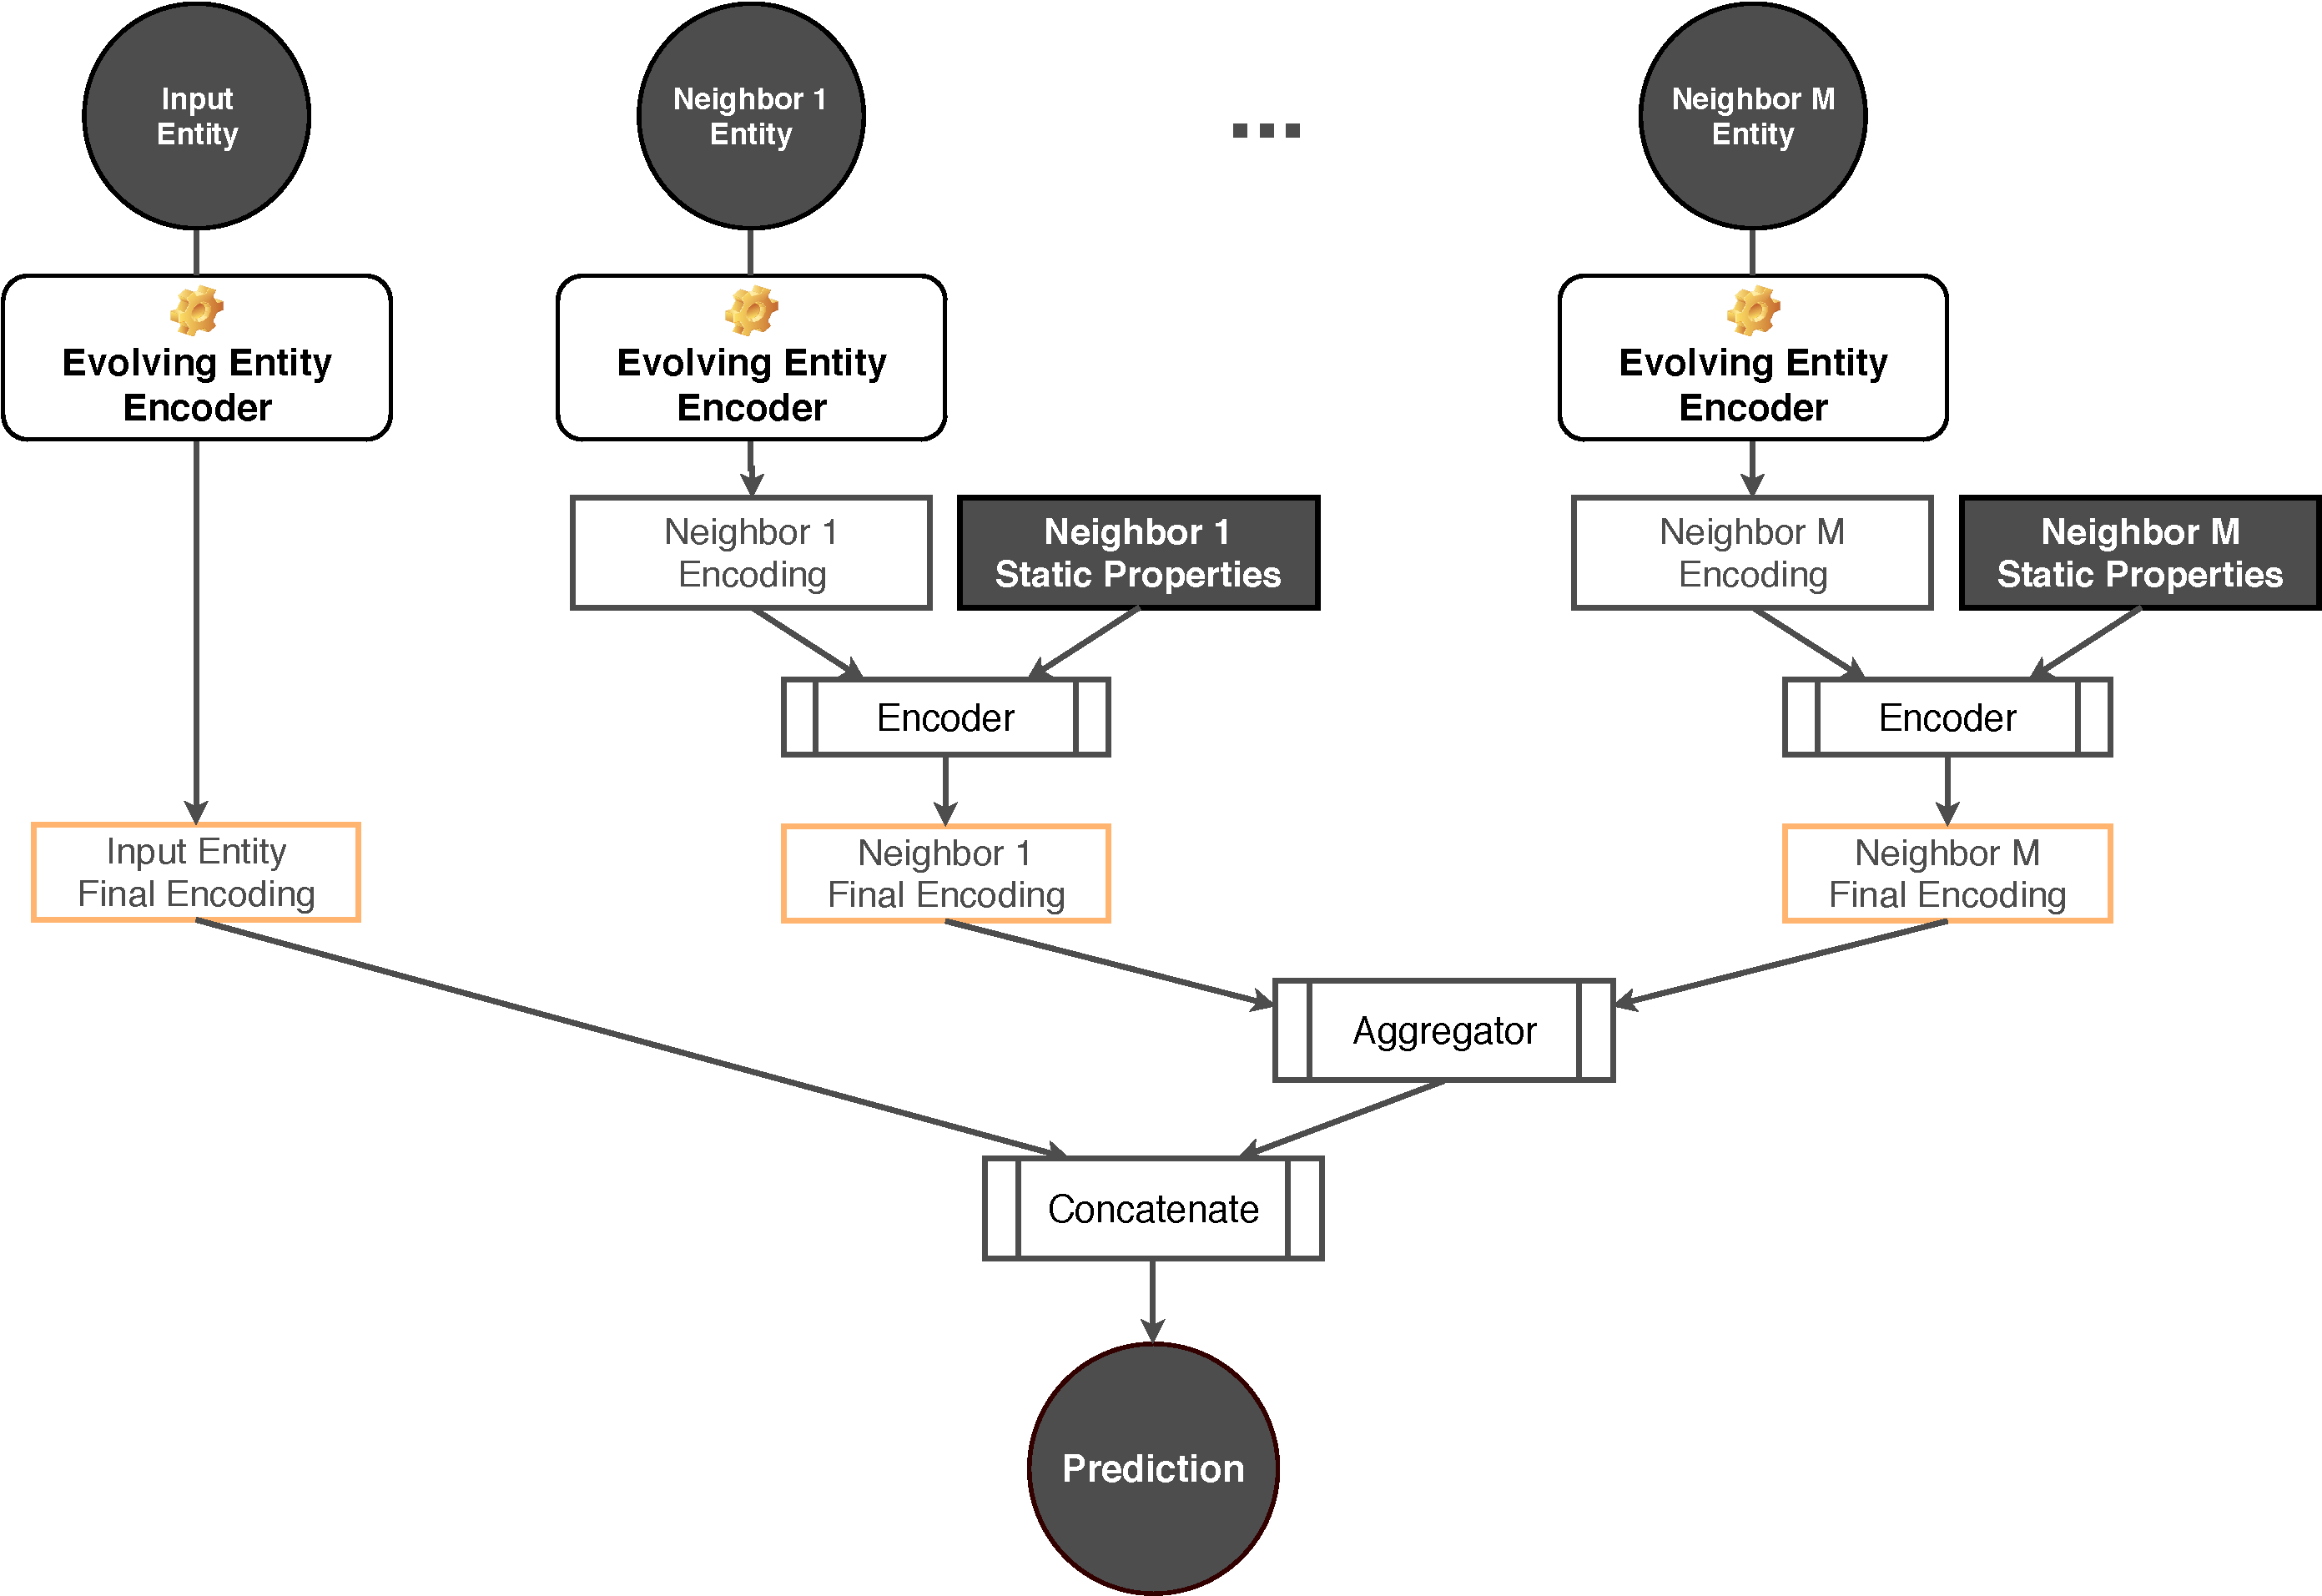
\includegraphics[width=0.7\textwidth]{figures/kg-rnn-general.pdf}
 \caption{The general module of our architecture, where \textbf{Evolving Entity Encoder} relies on work from previous chapter. The static properties and information from neighbors are concatenated and fed through an \emph{Encoder}, consisting of a simple fully-connected layers to blend the concatenated information. All encoding vectors from neighbors are aggregated along the $M$ dimension and concatenated with the input entity. This vector is then further fed into a fully-connected layer, here hidden in the \emph{Concatenate} block, to output the predictions.}
 \label{fig:kg-rnn-general}
\end{figure}

The following figure is a special case of the general approach available in the previous figure. Indeed, in our practical application we decided to get rid of the dynamic information from neighbors, leading to the following adapted schema:

\begin{figure}[H]
 \centering
 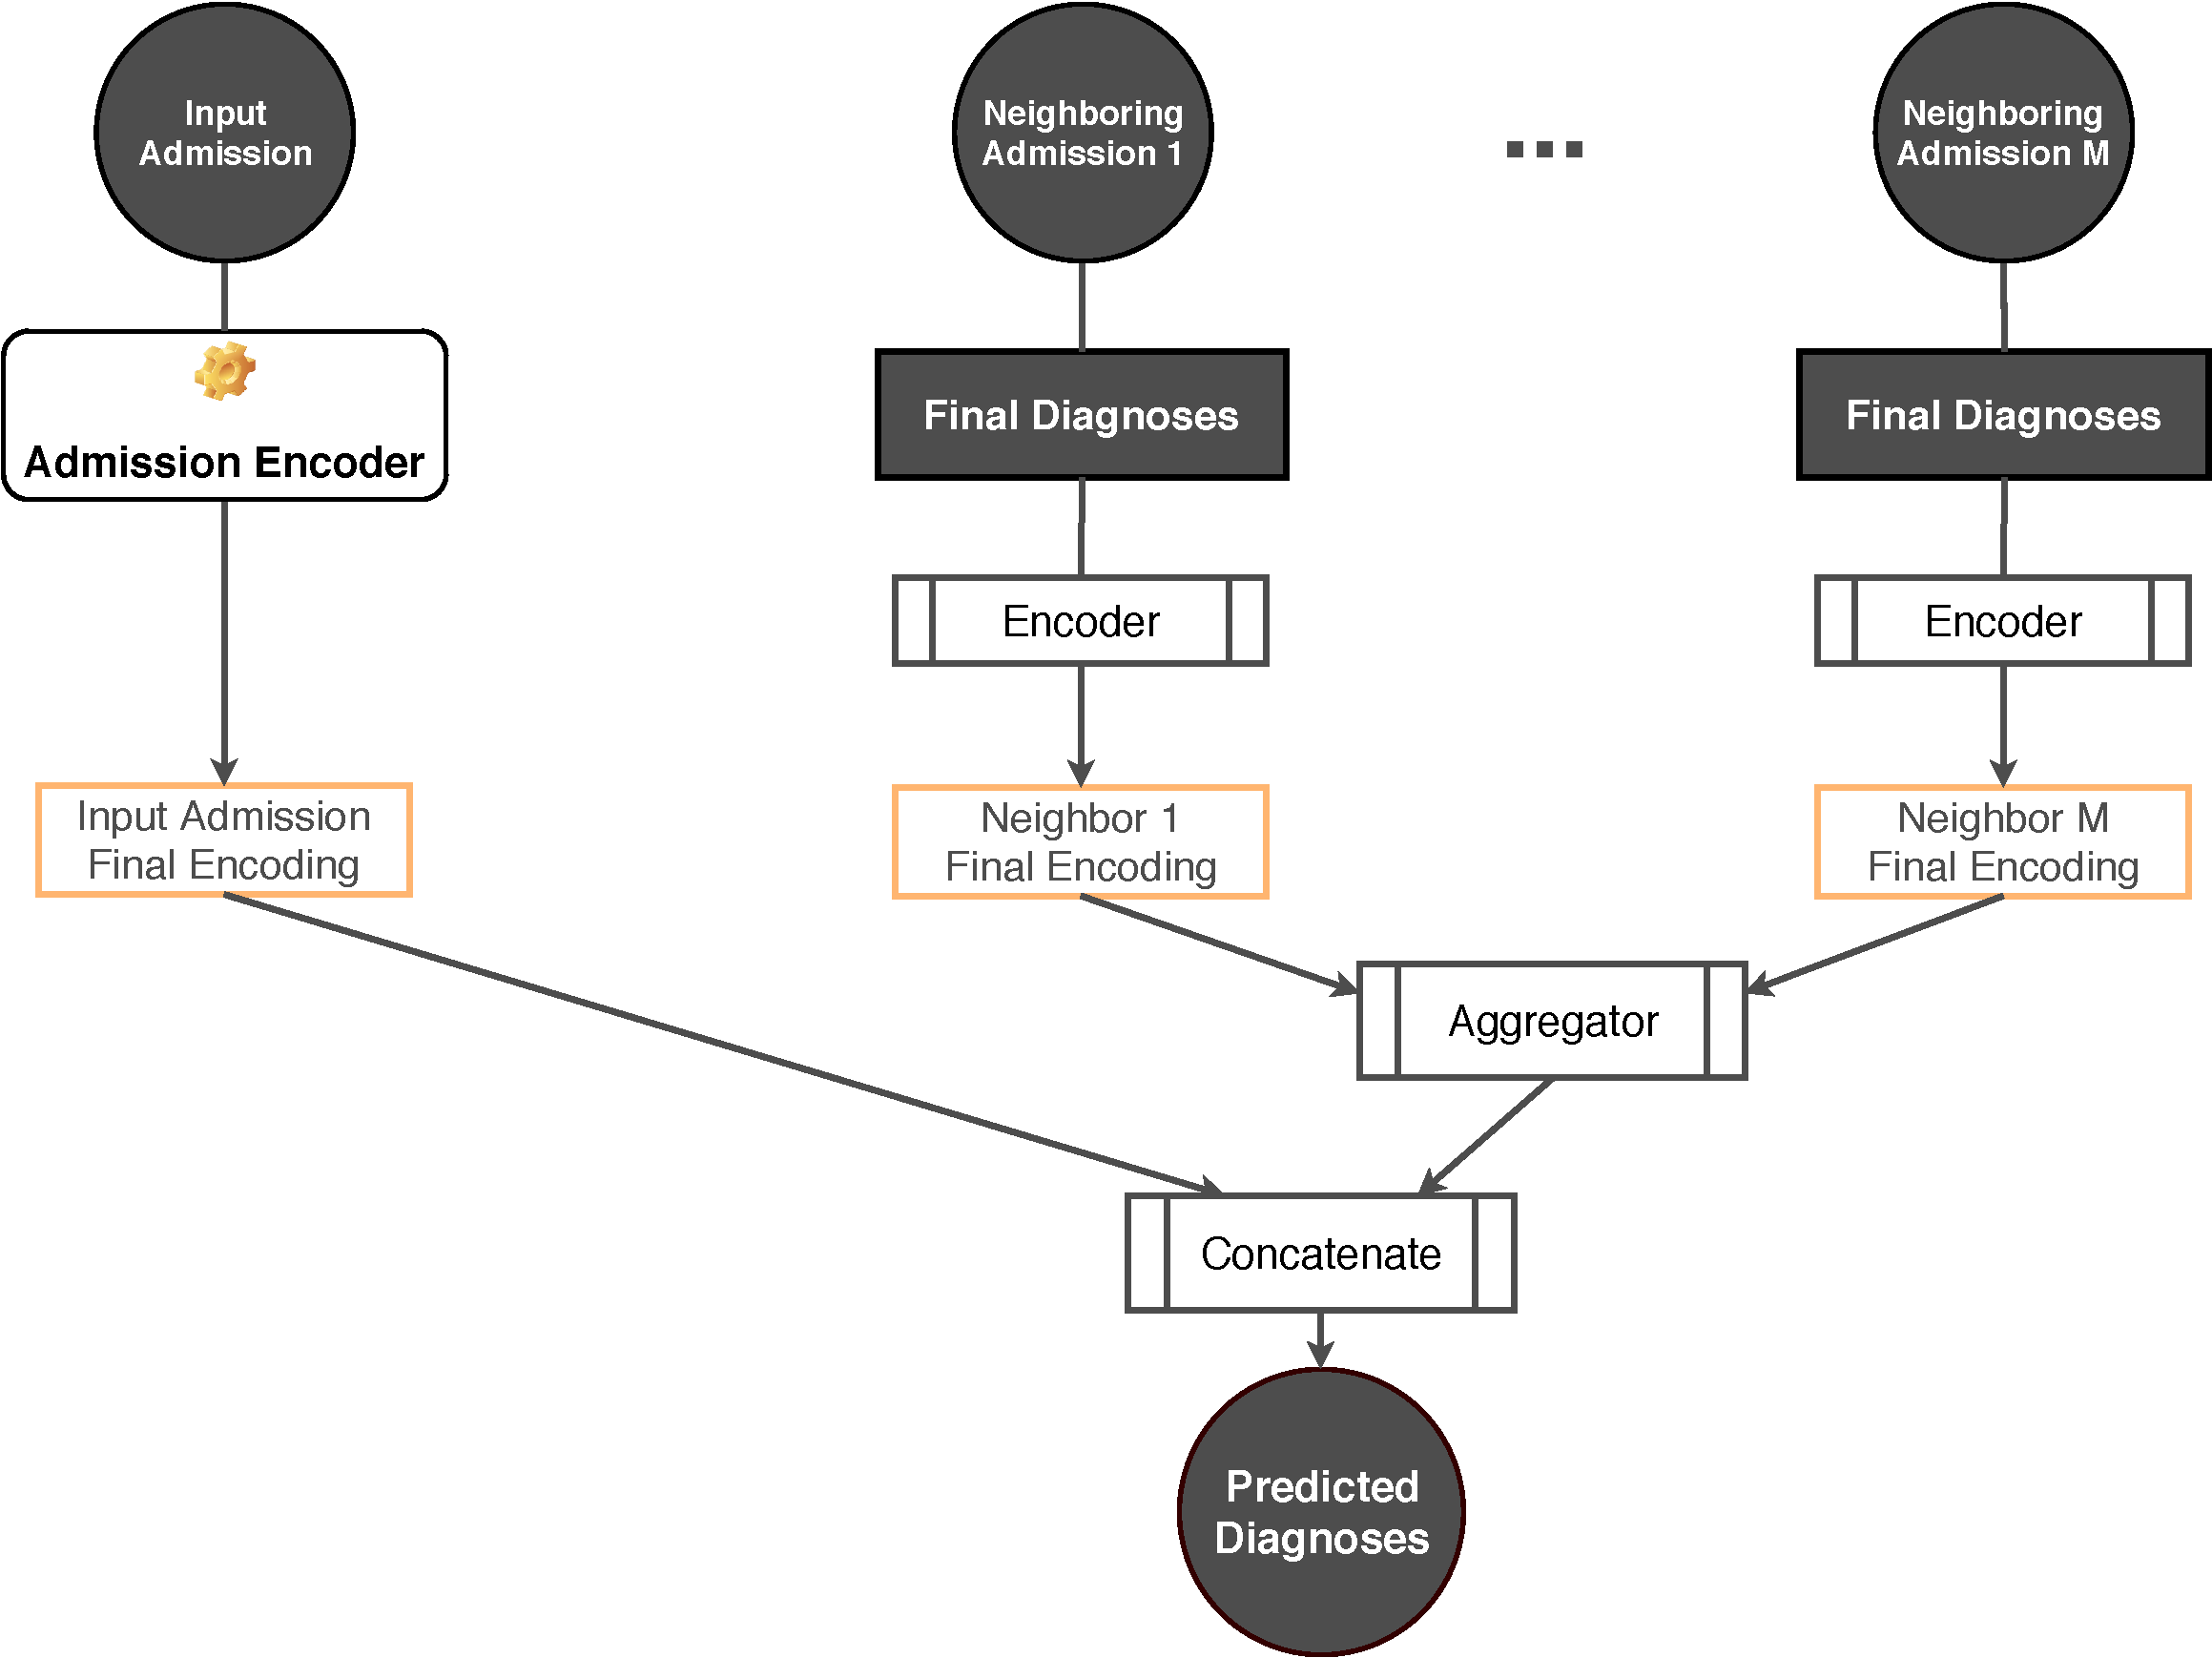
\includegraphics[width=0.6\textwidth]{figures/kg-rnn-healthcare.pdf}
 \caption{Similar to the previous schema, except that only static information from neighbors is encoded and squashed. Here the static information consist of only the diagnoses of these neighboring admissions.}
 \label{fig:kg-rnn-healthcare}
\end{figure}

As mentioned previously, in our case we decided to discard dynamic information from neighbors but we argue that this is heavily application-dependent, thus validating on different tasks and knowledge graphs would be insightful.